\documentclass[../thesis.tex]{subfiles}
\begin{document}

\section{Objective}\label{sec__intro__objective}
One of the most fundamental ways we can quantitatively analyse the world around us is through counting. 
It is one of the first abstract tasks we learn as children and it is simple to explain. To count is in effect to answer the question `How many instances are there of a given type?'. 
Even though the description of the task is simple and it is easy for humans to perform, it has broad and impactful applications in a variety of industries, including ecology with animal counting \cite{go2021fine, arteta2016counting}, urban planning with vehicle \cite{arteta2014interactive, Lu18, mundhenk2016large} and crowd counting \cite{wang2011automatic, wang2015deep, marana1997estimation, cao2018scale, barinova2012detection, Lu18}, and various medical and biological disciplines that require cell counting \cite{xie2018microscopy, morelli2021automating}. These industries would all benefit from being able to gather more accurate and reliable data in a shorter amount of time with less manual labour.
While modern machine learning systems are increasingly able to complete more and more complex tasks, they are still flawed in their ability to count, especially when the type and visual appearance of objects are not consistent between images.

This thesis furthers the abilities of automated enumeration methods.
Until recently, counting, in a machine-learning context, has been focused on individual, specific tasks. 
Often, counting methods were formulated as the classification or detection of a known kind of object.
While people may count in this way in simple, known cases, we believe that the human ability to count goes beyond this restricted approach.
When counting, a person does not have to check each pixel or object against a catalogue of all known kinds of objects. 
They can identify areas of interest that they believe could contain something `worth counting' and then draw comparisons between them. 
In this way, people are able to count instances of types of objects they have never seen before with limited-to-no guidance.

The work presented in this thesis is motivated by the desire to automate the human ability to count in novel situations with minimal guidance.
Foundational to our work is the intuition that human counting is comprised of two stages: object detection and repetition recognition.
See \Cref{fig__intro__intro_counting_image} for a visual representation of these two stages.
In this thesis, we first address these stages separately. We then develop methods which approach both stages simultaneously to gain a more holistic understanding of counting.

\begin{figure}
     \centering
     \begin{subfigure}{0.285\textwidth}
         \centering
        
\includegraphics[height=3.6cm]{../files/intro/teaser2__sub_0_a}
         \caption*{Input Image}
     \end{subfigure}
     \begin{subfigure}{0.285\textwidth}
         \centering
         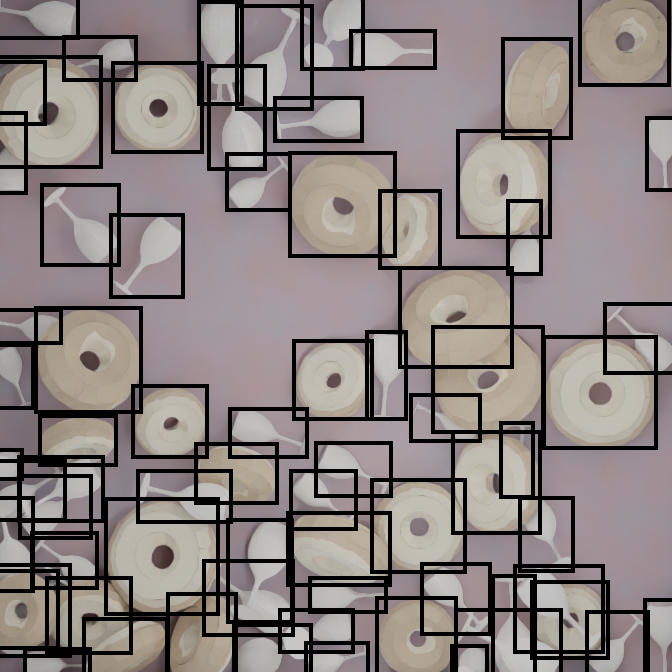
\includegraphics[height=3.6cm]{../files/intro/teaser2__sub_0_b}
         \caption*{Object Detection}
     \end{subfigure}
     \begin{subfigure}{0.285\textwidth}
         \centering
         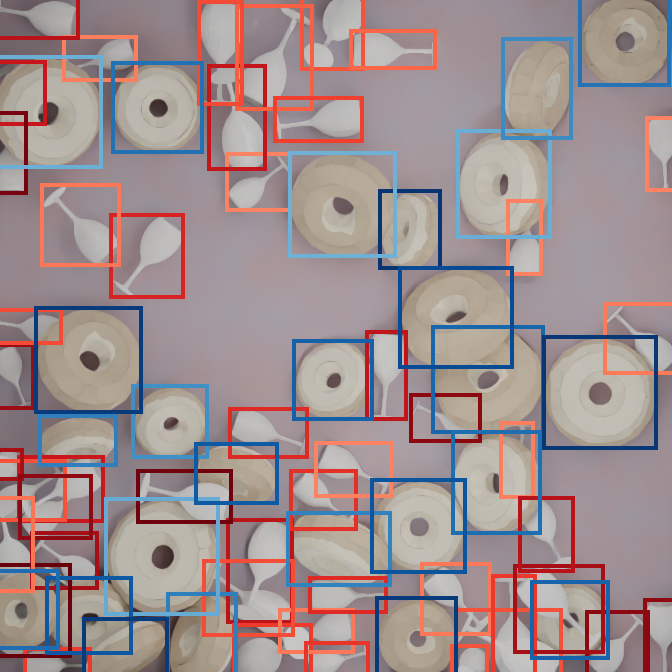
\includegraphics[height=3.6cm]{../files/intro/teaser2__sub_0_c}
         \caption*{Repetition Recognition}
     \end{subfigure}
     \begin{subfigure}{0.057\textwidth}
         \centering
         
\includegraphics[height=3.6cm]{../files/intro/Untitled drawing-29}
         \caption*{Counts}
     \end{subfigure}
        \caption{An example of the two  counting stages on a multi-class image from our dataset, MCAC. Areas that could be `worth counting' are located and compared to generate the final counts.}
        \label{fig__intro__intro_counting_image}
\end{figure}

\section{Thesis Structure and Contributions} 
In this section, we discuss the structure of this dissertation, outlining the context of each section and their contributions.

\textbf{\Cref{sec__literature_review}} provides context and motivation to our work as a whole. 
We first outline the important network architectures relevant to our work.
Then, we summarise the existing clustering and counting methods, provide an overview of their limitations, and discuss how they motivate our work.
The developments within the field of class-agnostic counting that occurred concurrent to our work are presented in the relevant chapters.

Throughout the work presented in this dissertation, we encountered errors, ambiguities, and limitations of the most popular class-agnostic counting dataset, FSC-147. In \textbf{\Cref{sec__Datasets}}, we address these and present FSC-133, an improved version of the popular dataset without those errors or ambiguities.
This improved dataset enables more effective training of class-agnostic counting methods and, more importantly, more accurate evaluation of them.
We then go on to discuss the need for a new dataset to enable the training and evaluation of class-agnostic counting methods in settings with multiple objects and explain why a synthetic dataset is the most appropriate choice for this setting.
We then present the first Multi-class Class-Agnostic Counting dataset (MCAC).
Both FSC-133 and MCAC are used in \Cref{sec__LTCA,,sec__ABC123} to train and validate our methods, as well as those of our contemporaries.

In \textbf{\Cref{sec__DMS}}, we concentrate on the repetition recognition stage of counting, separate from the detection stage.
We address the question `Given a set of single instances, how many are there of each type?' by framing it as a clustering problem.
We recognise that to function robustly,  many of the previous clustering approaches require complex or large-scale parameter tuning. 
This tuning often requires information such as the number of clusters present in the dataset or some form of distance metric to define the boundary between points which are similar or dissimilar.
This prior knowledge is often difficult to gather or completely unknown, and parameters used to define similarity in classical methods do not generalise well to high dimensional spaces.
These earlier clustering methods also generally divide a set of points in a single way.
We observe that, in many cases, there are numerous ways to group a set of data points depending on the features relevant to a given task. A method capable of addressing this complexity would be highly beneficial.
We believe that the ability of machine learning methods to identify trends as well as function in high-dimensional feature spaces will enable a flexible clustering method which can solve varied clustering problems with much less contextual information than previous methods.

To this end, we developed a Differentiable Mean Shift algorithm (DMS). This iterative neural network mirrors the traditional Mean-Shift algorithm in a fully differentiable way by gradually improving its understanding of cluster centres. DMS is trained using small amounts of `side-information' in the form of pairwise `similar/dissimilar' labels.
DMS is able to cluster the same set of features in different ways depending on the side-information provided. This enables it to be task-specific, identifying groupings that are not the most obvious, while still requiring minimal human input.
While we present this work mostly in the context of clustering images based on various visual features, it could be applied to any feature space or task.
As DMS is completely differentiable, it can be used within other end-to-end trainable methods as well as a stand-alone clustering method.


While  \Cref{sec__DMS} focused on solely the repetition recognition half of the counting problem, \Cref{sec__LTCA,,sec__ABC123} address both the object detection and repetition in tandem, creating complete instance counting methods.

Traditionally, counting methods are class-specific; methods would be trained to count occurrences of a specific object in an image. Class-agnostic methods aim to count objects of any type. 
Class-agnostic counters should be able to function in much more varied contexts than class-specific ones without the need for retraining, removing the requirement for large amounts of training data of each kind of object during deployment.

Prior to our work, class-agnostic counting methods required intervention, in the form of exemplar images, during training and at inference time. The exemplar images are used to define the type of object to be counted.
In many contexts, including those presented in the main class-agnostic counting dataset, we do not think this is necessary.
Presented with an image containing only one kind of object and asked to `count', a person understands the task at hand, even if the object class is novel. 
In \textbf{\Cref{sec__LTCA}}, we introduce RCC, a class-agnostic counter that operates without the need for exemplars, marking the first instance of a method replicating this behaviour.
Not only can RCC count without needing exemplar images at training or inference time, but it can also be trained using only scalar image-wise counts as supervision rather than using instance-wise locational labels. 
RCC achieves results competitive with prior and concurrent class-agnostic counting methods that use exemplar images and that train with instance-wise labels.

The work in \Cref{sec__LTCA} shows that the human ability to perform `uninformed counting' is automatable in single-class settings.
However, we recognise that many real-world applications do not have the known constraint that only a single kind of object will be present in each image while also not knowing the object class.
Similar to our observation about the ability of humans to perform uninformed counting in single-class settings, we believe that people can, in general, count objects of multiple types in an image without being told the class boundaries or being given exemplars of type.
We show in this thesis that this behaviour is replicable in an automated system.


In \textbf{\Cref{sec__ABC123}}, we present A Blind Counter (ABC123) the first multi-class exemplar-free class-agnostic counter. 
ABC123 can count instances of multiple types simultaneously without human intervention.
While it is generally hypothesised that exemplar-based methods should function well in multi-class settings, using the exemplar images to clarify ambiguities, this has not been shown robustly.
Using MCAC, we demonstrate that many pre-existing methods perform poorly in multi-class settings and that ABC123 performs well in them.
We also demonstrate that the understanding of counting learnt from MCAC, a synthetic dataset, is transferable to photographic data.


\textbf{\Cref{sec__conclusion}} provides an overview of the research presented in this thesis, emphasising our contributions. Additionally, we explore and discuss potential directions for future research.



\section{Publications and Public Releases}
\looseness=-1 Here, we present the publications and public releases of the work included in this thesis:

\begin{itemize}
    \item \textbf{M. Hobley}, and V Prisacariu. ``DMS: Differentiable Mean Shift for Dataset Agnostic Task Specific Clustering Using Side Information.'' Completed in 2019, \textit{ArXiv e-prints}. 2023.
    \item \textbf{M. Hobley}, and V Prisacariu. ``Learning to count anything: Reference-less class-agnostic counting with weak supervision.'' Completed in 2022, in the \textit{Proceedings of the Conference on Computer Vision and Pattern Recognition}. 2023.
    \item \textbf{M. Hobley}, and V Prisacariu. ``ABC Easy as 123: A Blind Counter for Exemplar-Free Multi-Class Class-agnostic Counting'' \textit{ArXiv e-prints}. 2023. Currently Under Review for the \textit{Conference on Computer Vision and Pattern Recognition}. 2024.
\end{itemize}



\end{document}